\section{Constraint Satisfaction}

This section maps the project handout constraints and course rubric to concrete implementation evidence in the repository. Narrative report requirements (context, collaboration, challenges, individual contributions, and lessons learned) are developed in Sections~1, 4, 5, and~6; here we focus on \emph{technical} constraint satisfaction with file-level traceability.

\subsection{Constraint-to-evidence matrix}
Table~\ref{tab:constraint_evidence} is the primary traceability artifact: each row states a constraint, how the codebase satisfies it, where to inspect the implementation, and the observable outcome.

% [H] pins the float here so §3.2+ do not typeset before Table~\ref{tab:constraint_evidence}.
\begin{table}[H]
    \centering
    \footnotesize
    \caption{Mapping of project constraints to implementation evidence.}
    \label{tab:constraint_evidence}
    % Relax line-breaking; paths break at slashes/underscores with xurl.
    \begingroup
    \sloppy
    \emergencystretch=4em\relax
    % Full portrait text width; middle column (Evidence) is widest (\hsize factors sum to 3).
    \begin{tabularx}{\textwidth}{@{} >{\raggedright\arraybackslash}p{2.2cm} >{\raggedright\arraybackslash\hsize=0.85\hsize}X >{\raggedright\arraybackslash\hsize=1.35\hsize}X >{\raggedright\arraybackslash\hsize=0.80\hsize}X @{}}
        \toprule
        \textbf{Constraint} & \textbf{Approach} & \textbf{Evidence (representative paths)} & \textbf{Outcome} \\
        \midrule
        File input/output (text + binary) &
        Read JSON, WAV, BMP; write plain render log (text), compressed container (mixed text header + binary payloads), optional process log. &
        \url{src/parsers/json/json.c}, \url{src/parsers/wav.c}, \url{src/parsers/bmp.c}; \url{src/components/render.c}, \url{src/components/render_compress.c}; \url{src/components/engine.c}; \url{src/components/preview.c}. &
        Deterministic artifacts: render text, compressed output, log. \\
        \addlinespace
        Custom robust parser(s) &
        Dedicated parsers with typed errors; config layer whitelists keys and validates ranges; engine rejects unknown compression strings. &
        \url{src/parsers/json/config.c} (allowed keys, required fields, defaults); \url{src/parsers/json/json.c}; \url{src/parsers/wav.c}; \url{src/parsers/bmp.c}; \texttt{engine\_prepare\_compression} in \url{src/components/engine.c}. &
        Invalid files or config fail early with explicit error codes instead of silent corruption. \\
        \addlinespace
        Clean C + strict warnings &
        Project build uses strict GCC flags for all translation units and tests. &
        \texttt{Makefile} (\texttt{CFLAGS = -Wall -Werror -ansi -pedantic -Iinclude}). &
        Warning-free, standards-oriented compilation baseline. \\
        \addlinespace
        State machines &
        Engine runtime is a finite state machine over load, prepare, compress-prep, output, frame loop, and summary stages; Huffman decoding uses an explicit FSM table; preview parses header and frame records sequentially. &
        \texttt{engine\_run} and \texttt{EngineState} in \url{src/components/engine.c}; \texttt{huffman\_build\_fsm} / FSM types in \url{src/compressions/algorithms/huffman.c} and \url{include/compressions/algorithms/huffman.h}; \texttt{parse\_header}, \texttt{parse\_fsm}, \texttt{read\_frame} in \url{src/components/preview.c}. &
        Clear control flow, stage isolation, and decode structure suitable for complex I/O. \\
        \addlinespace
        Parser complexity &
        Multiple non-trivial parsers: JSON subset + config semantics; RIFF/WAVE PCM; BMP DIB/pixel layout; compressed-file header and per-frame records in preview. &
        As above, plus \url{include/parsers/json/json.h}, \url{include/parsers/wav.h}, \url{include/parsers/bmp.h}, \url{include/components/render_compress.h}. &
        Demonstrates layered parsing beyond a single trivial format. \\
        \addlinespace
        No external libraries &
        Implementation uses ISO C standard library; preview uses conditional POSIX vs.\ Windows calls for timing and screen clear, not third-party frameworks. &
        \texttt{Makefile} link lines; \texttt{\#ifdef \_WIN32} branches in \url{src/components/preview.c}. &
        Self-contained build without dependency managers or non-standard SDKs. \\
        \addlinespace
        Code quality + feature depth &
        Modular boundaries (parsers, components, compressions, tests); multiple compression modes (\texttt{none}, \texttt{rle}, \texttt{delta}, \texttt{huffman}) integrated through \texttt{compress\_frame} / \texttt{decompress\_frame}. &
        \url{src/compressions/compress.c}, \url{src/compressions/decompress.c}; \url{src/compressions/algorithms/} (\texttt{*.c}); \url{tests/parsers}, \url{tests/components}, \url{tests/compressions}. &
        Maintainable structure with substantive algorithmic content. \\
        \bottomrule
    \end{tabularx}
    \endgroup
\end{table}

\subsection{File input and output in detail}
\textbf{Inputs.} Configuration is a JSON object loaded by \texttt{config\_load} (\url{src/parsers/json/config.c}), which requires keys such as \texttt{frames\_dir}, \texttt{fps}, frame range, \texttt{palette}, \texttt{threshold}, and \texttt{compression\_algorithm}, with optional \texttt{huffman\_K} and frame-naming fields. Audio is read as a binary WAV (\url{src/parsers/wav.c}). Frames are read as BMP files (\url{src/parsers/bmp.c}) along paths built by \texttt{sequence\_build\_frame\_path} (\url{src/components/sequence.c}).

\vspace{0.3em}
\noindent \textbf{Outputs.} The engine writes a human-readable ASCII timeline via \texttt{render\_write\_frame} (\url{src/components/render.c}), a compressed stream via \texttt{render\_write\_header} and \url{render_write_frame_compressed} (\url{src/components/render_compress.c}), and a textual process log. The \texttt{preview} program opens the compressed file in binary mode, parses textual header lines and embedded FSM metadata when applicable, reads binary frame payloads, and prints decoded ASCII (\url{src/components/preview.c}).
This satisfies the handout requirement for file-based processing across both text and binary modalities.

\vspace{0.5em}
\noindent \textbf{Compressed Output Format.}  

\noindent The compressed file follows a hybrid \textbf{text + binary} format. The header is stored as human-readable text, followed by optional FSM metadata (for Huffman), and then per-frame binary payloads.

\vspace{0.3em}
\noindent \textbf{Header.}  
The file begins with global metadata:
\begin{itemize}
    \item \texttt{FORMAT}: file identifier (e.g., ASCII\_VIDEO)
    \item \texttt{WIDTH}: frame width 
    \item \texttt{HEIGHT}: frame height
    \item \texttt{COMPRESSION}: compression type identifier (0: None, 1: RLE, 2: Delta, 3: Huffman)
    \item \texttt{K}: number of bits processed per step in the Huffman FSM (only applicable when Huffman compression is used)
    \item \texttt{NUM\_STATES}: number of FSM states
\end{itemize}

\vspace{0.3em}
\noindent \textbf{FSM Section (Huffman only).}  
If Huffman compression is used, the FSM is serialized between \texttt{FSM\_BEGIN} and \texttt{FSM\_END}. Each line represents one transition:
\[
\texttt{state\;\;input\;\;next\_state\;\;bits\_used\;\;output\_length\;\;[symbols...]}
\]
where:
\begin{itemize}
    \item \texttt{state}: current FSM state
    \item \texttt{input}: $K$-bit input (as integer)
    \item \texttt{next\_state}: next FSM state
    \item \texttt{bits\_used}: number of bits consumed
    \item \texttt{output\_length}: number of decoded characters
    \item \texttt{symbols}: ASCII values of output characters, separated by spaces; `-` if \texttt{output\_length} is 0
\end{itemize}

\vspace{0.3em}
\noindent \textbf{Frame Section.}  
Each frame is stored with metadata followed by compressed binary data:
\begin{itemize}
    \item \texttt{FRAME}: frame index
    \item \texttt{TIME}: timestamp
    \item \texttt{DATA\_BITS}: number of valid bits in the payload
    \item \texttt{DATA\_BEGIN} / \texttt{DATA\_END}: delimit binary data
\end{itemize}

\noindent The actual compressed data is stored as a packed bit stream, where bits are written into bytes and read using a bit-level reader during decoding.

\vspace{0.3em}
\noindent \textbf{Design Rationale.}  
This format separates structure from data: textual headers and FSM metadata provide readability, while binary payloads ensure compact storage. The FSM representation allows efficient decoding without reconstructing the Huffman tree, enabling fast multi-bit processing during playback.


\noindent These satisfy the handout requirement for file-based processing across both text and binary modalities.


\subsection{Parser robustness and incorrect-input detection}
Robustness is implemented through \emph{validation at boundaries} and \emph{typed error returns} rather than ad-hoc crashes:

\begin{itemize}
    \item \textbf{JSON and config:} unknown keys are rejected (\texttt{config\_validate\_allowed\_keys}); required keys must be present and correctly typed; string length and numeric ranges are checked (\texttt{config\_validate}). Frame extension is restricted to \texttt{.bmp} and \texttt{frame\_digits} is capped, preventing ambiguous or oversized paths.
    \item \textbf{WAV and BMP:} parsers verify signatures, header consistency, and supported format assumptions appropriate to the course scope (PCM WAV; uncompressed BMP suitable for the frame pipeline).
    \item \textbf{Compression selection:} strings other than \texttt{none}, \texttt{rle}, \texttt{delta}, and \texttt{huffman} fail in \texttt{engine\_prepare\_compression}; Huffman additionally requires \texttt{huffman\_K > 0} (\url{src/components/engine.c}).
\end{itemize}

Table~\ref{tab:parser_faults} summarizes typical fault categories and the defensive response pattern (exact error codes are enumerated in the respective headers under 
\url{include/parsers/} and \url{include/components/}).

\begin{table}[H]
    \centering
    \small
    \caption{High-level parser fault categories and system response.}
    \label{tab:parser_faults}
    \begin{tabular}{@{}p{0.28\linewidth} p{0.32\linewidth} p{0.34\linewidth}@{}}
        \toprule
        \textbf{Fault category} & \textbf{Example} & \textbf{Response pattern} \\
        \midrule
        Structural / syntax & Invalid JSON; malformed WAV/BMP headers &
        Parse fails; \texttt{config\_load} or low-level parser returns non-success; engine aborts in error state. \\
        \addlinespace
        Schema / policy & Unknown config key; wrong value type; invalid frame range &
        \texttt{CONFIG\_ERR\_UNKNOWN\_KEY}, \texttt{CONFIG\_ERR\_WRONG\_TYPE}, or range errors; safe re-init of config. \\
        \addlinespace
        Unsupported media & Non-conforming BMP or WAV for implemented subset &
        Load error at BMP/WAV layer; engine surfaces failure without emitting partial outputs. \\
        \addlinespace
        Invalid compression mode & Unrecognized \texttt{compression\_algorithm} string &
        \texttt{ENGINE\_ERR\_CONFIG} from \texttt{engine\_prepare\_compression}. \\
        \bottomrule
    \end{tabular}
\end{table}

Automated tests under \url{tests/parsers}, \url{tests/components}, and \url{tests/compressions} exercise many negative paths; full end-to-end engine tests are lighter and remain a documented improvement opportunity (Section~6).

\subsection{Constraint pipeline (diagram)}
Table~\ref{tab:constraint_evidence} is intentionally dense; Figure~\ref{fig:constraint_pipeline} gives the same end-to-end structure in visual form: heterogeneous inputs, parser layer, engine and rendering, compressed output, and preview playback.

\begin{figure}[htbp]
    \centering
    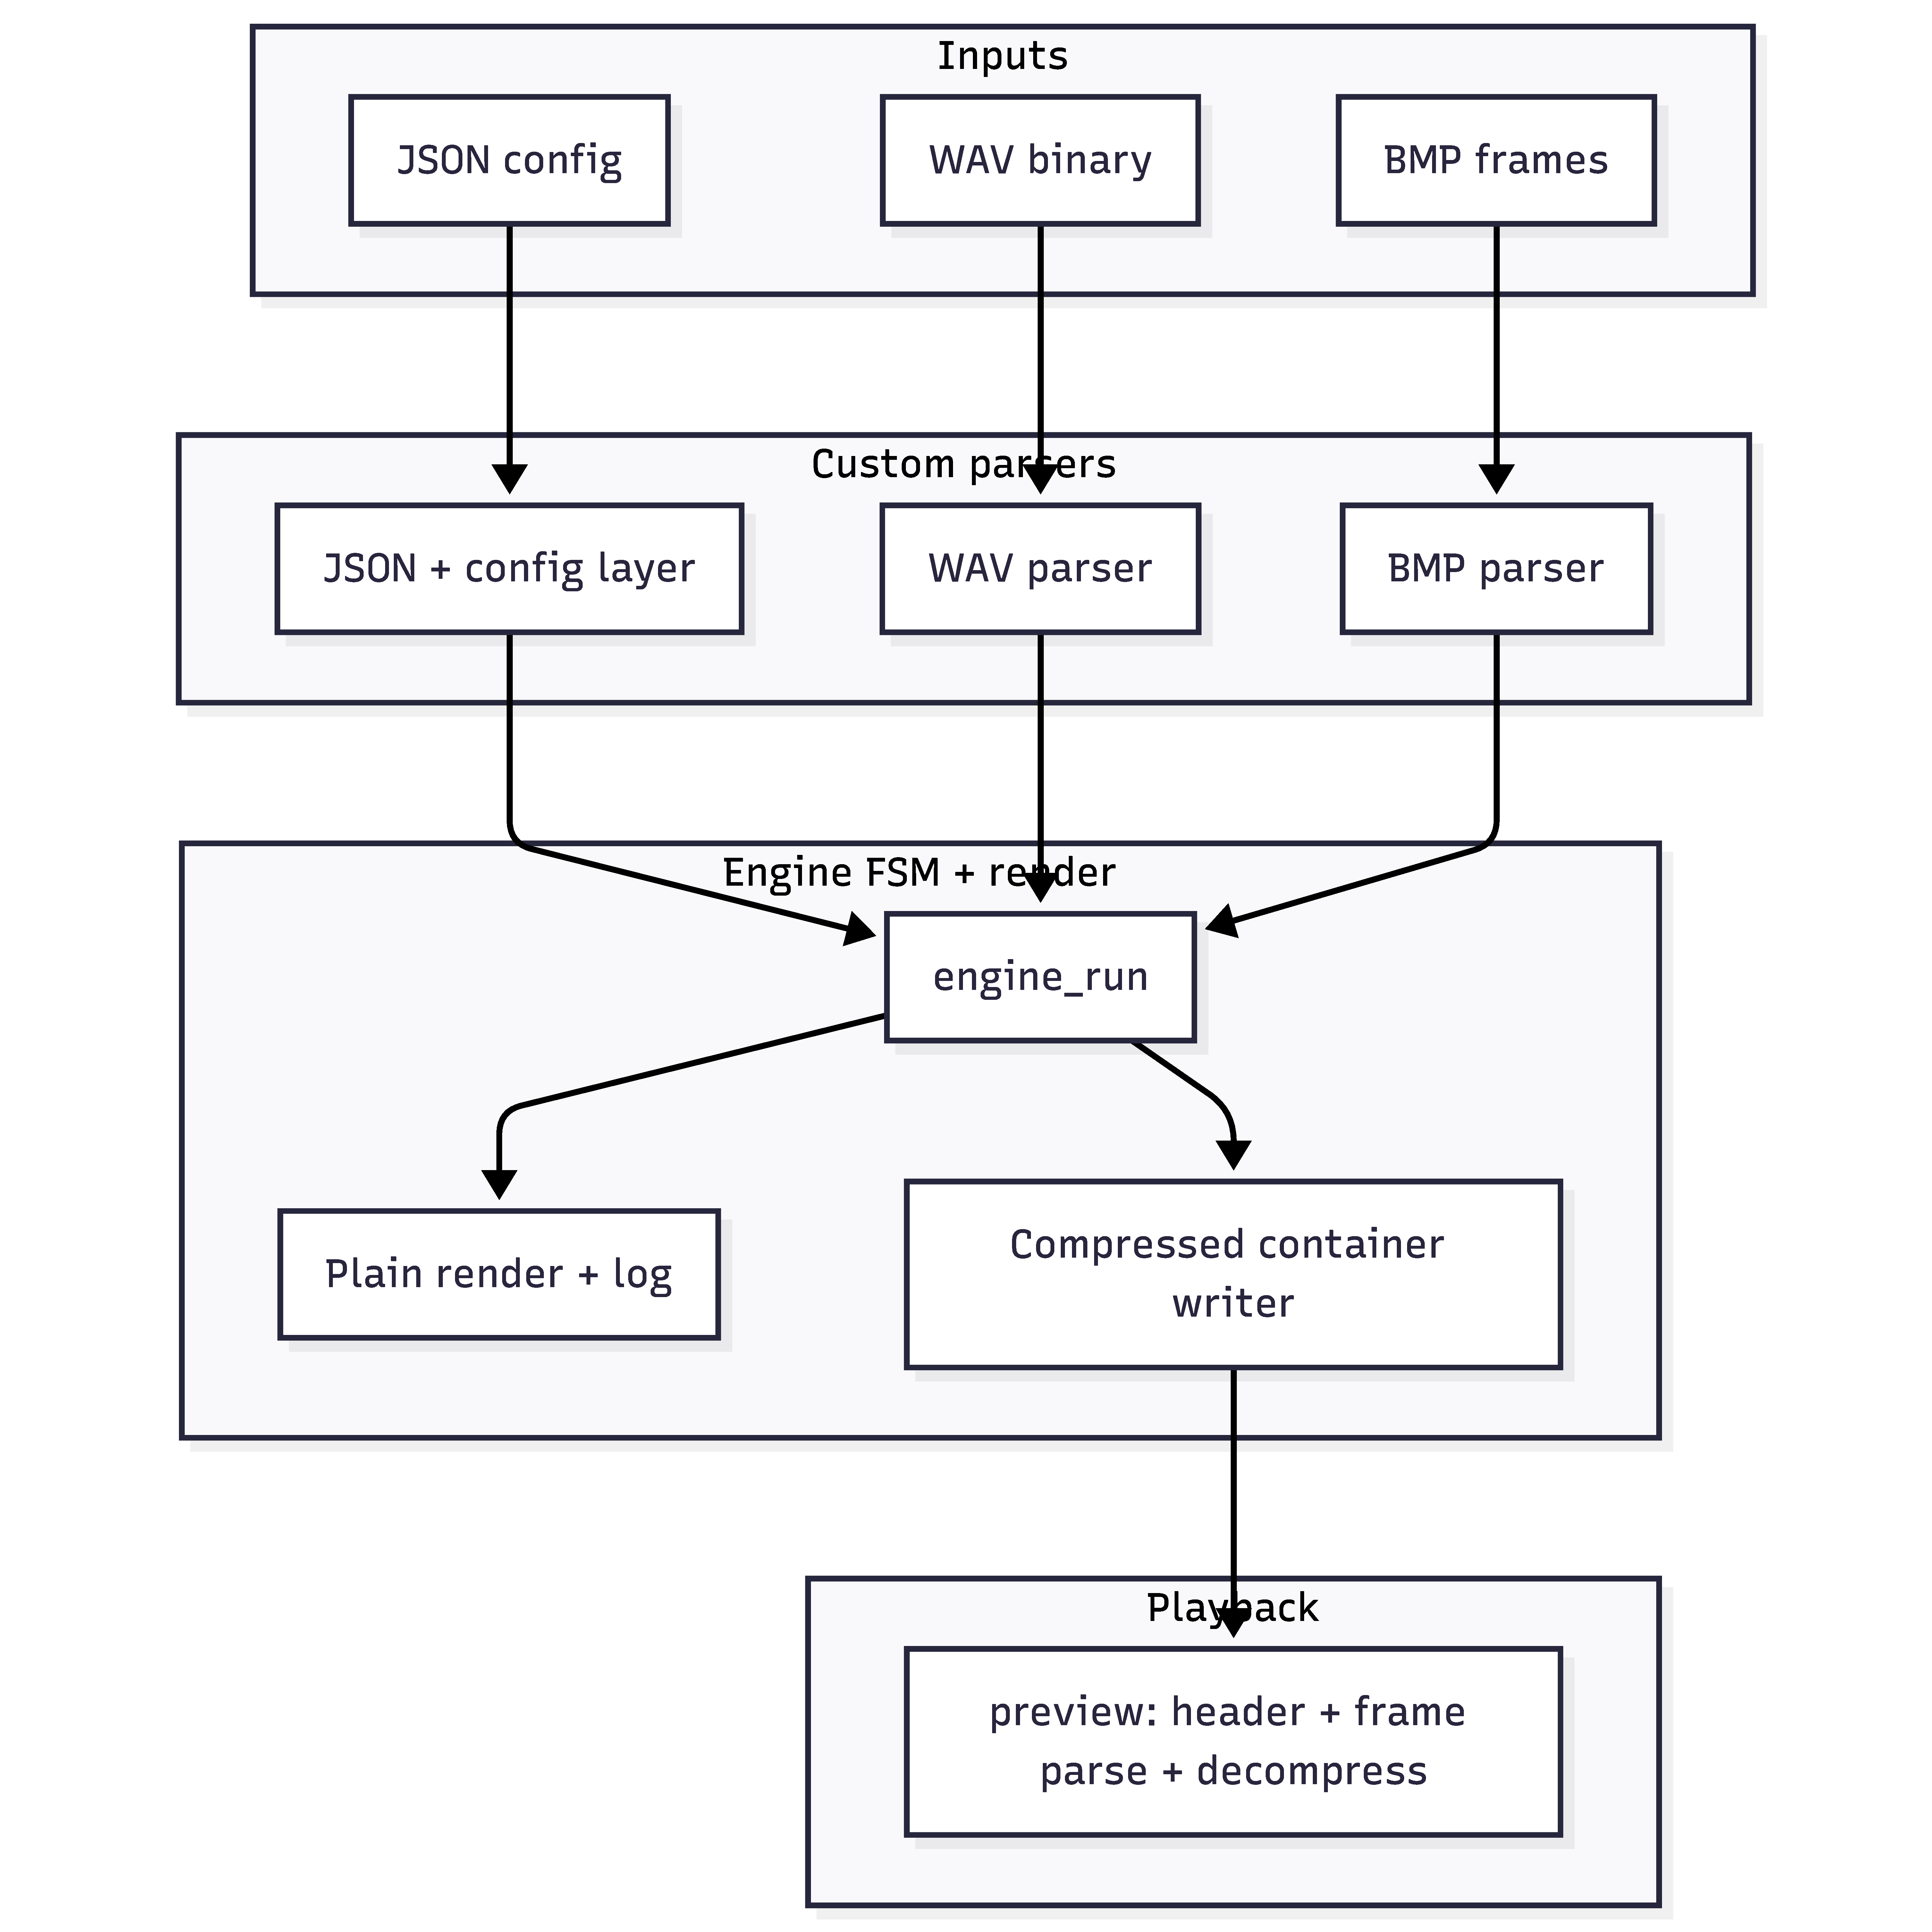
\includegraphics[width=\textwidth]{figures/data_flow.pdf}
    \caption{High-level data flow and rubric-oriented module boundaries: inputs through parsers and engine to plain and compressed outputs, then preview. Complements the constraint-to-evidence matrix in \S~3.1.}
    \label{fig:constraint_pipeline}
\end{figure}
